\documentclass{article}
\usepackage[utf8]{inputenc}
\usepackage{tikz}
\usepackage{standalone}
\usepackage{amsmath}
\usepackage{amsfonts}
\usepackage[a4paper, total={7.5in, 10in}]{geometry}
\usepackage{hyperref}
\usepackage{pbox}

\usepackage{tikz}
\usetikzlibrary{shapes.geometric}
\usepackage{standalone}
\usepackage{graphicx, color}


\newcommand{\bA}{\mathbf{A}}
\newcommand{\bB}{\mathbf{B}}
\newcommand{\bC}{\mathbf{C}}
\newcommand{\bD}{\mathbf{D}}
\newcommand{\E}{\mathbb{E}}
\newcommand{\f}{\mathbf{f}}
\newcommand{\bg}{\mathbf{g}}
\newcommand{\bh}{\mathbf{h}}
\newcommand{\bL}{\mathbf{L}}
\newcommand{\Loss}{\mathcal{L}}
\newcommand{\bM}{\mathbf{M}}
\newcommand{\bN}{\mathbf{N}}
\newcommand{\Norm}{\mathcal{N}}
\newcommand{\R}{\mathbb{R}}
\newcommand{\bt}{\mathbf{t}}
\newcommand{\bU}{\mathbb{U}}
\newcommand{\bu}{\mathbf{u}}
\newcommand{\bw}{\mathbf{w}}
\newcommand{\bX}{\mathbf{X}}
\newcommand{\bx}{\mathbf{x}}
\newcommand{\by}{\mathbf{y}}
\newcommand{\bZ}{\mathbf{Z}}
\newcommand{\bz}{\mathbf{z}}

\begin{document}
\section*{Discussion points}

\subsection*{Is it plausible that the complexity of the IHDP dataset has been exhausted by our and earlier models?}
We had this question about the Infant Health and Development Program dataset and were wondering if it was a plausible theory. The problem is that there are multiple possible factors that lead to variance in the results. So far, it seems the model by Christos Louizos and our potential improvement on it score roughly the same, and better or similar to other papers. Our main question is: Is it plausible that a potential limit on the dataset is reached and that we shouldn't invest more time in improving scores on the IHDP dataset?

Some considerations on the dataset:
The dataset itself is semi-synthetic, which in this case means that the values that we want to predict are generated by a stochastic process. The dataset itself contains 747 samples and it seems common in the literature to use ten outcomes of the data generation process. This gives 7470 samples, kept separate in ten parts, allowing researchers to train their model ten times and aggregate the results in some way. 

There seems to be a significant difference between these ten 'versions' of the dataset. The value we want to predict has a different range between versions and can be up to an order of magnitude larger. From what I gather, most papers average the result over these ten versions, but it isn't entirely clear if all papers do that. It might be that some add all samples together into one dataset. In our case that makes the scores worse.


\subsection*{Does our idea of a new image-based dataset add something useful to causal inference research?}
In Figure \ref{fig:my_label} we have a sample of our proposed dataset. The image itself is in this case the covariate features/proxy variable and the intervention/action is the steering of the red circle. Latent factors are 'gravity' forces that influence the actual movement of the red circle. The value that the model should predict is how close the red circle gets to the center right position in the image. This is of course influenced by the original position of the red circle and the direction and magnitude of the steering vector but also by the latent gravity effect.

To evaluate the model we propose an adaptation of the $ITE$ (and $ATE$) scores. To do this we first rephrase them such that the two intervention values that are compared are now drawn from a delta distribution. Now we replace the two delta distributions by two other distributions over the intervention variable and we have a new effect we can measure on a dataset:
\begin{align}
    ITE(x) &:= \E[\by | \bX=x, do(\bt=1)] - \E[\by | \bX=x, do(\bt=0)]\\
    ITE(x) &:= \E[\by | \bX=x, do(\bt=t_1)] - \E[\by | \bX=x, do(\bt=t_0)], \quad t_1 \sim \delta_1, \quad t_0 \sim \delta_0\\
    ITE(x) &:= \E[\by | \bX=x, do(\bt=t_1)] - \E[\by | \bX=x, do(\bt=t_0)], \quad t_1 \sim p_{optimal}(t), \quad t_0 \sim p_{control}(t)
\end{align}
What $p_{optimal}$ and $p_{control}$ should be is somewhat open ended and we are wondering if it matters much if we are only interested in the RMSE between the real $ITE$ and the predicted $ITE$, give that they are distinct from each other.

\begin{figure}[h]
    \centering
    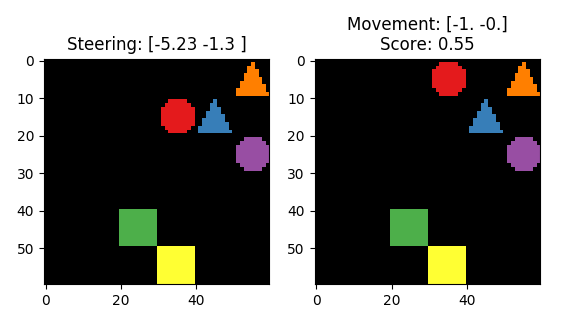
\includegraphics[width=0.7\textwidth]{latex/Figures/sample_space_shapes_with_score.png}
    \caption{Sample of the dataset. Image on the left, steering and the score are observed, rest is latent. The image on the right is given as visualisation of the final outcome.}
    \label{fig:my_label}
\end{figure}

\end{document}